\chapter{Implementation and Results}\label{chapter:implementation}

This chapter records the implementation of the trust-calibrated deliberation framework and the results available at the time of writing. It separates three kinds of evidence. The first is what ran on real hardware: Gate~0, a vanilla multi-agent debate on ten GPQA questions, a small live smoke of the optional B7 ceiling, the 4-bit N1a smoke, the FP8 precision smoke, and the first completed Core row (B8 trust versus the B8-no-trust majority control on GPQA-Main, seed~1). The second is what the P0 gate checks without a GPU: option rendering, answer parsing, trust bounds, endpoints, dataset pins, claim routing, the manifest guard, and the matrix budget. The third is the test suite, which exercises the same modules on synthetic and mock inputs. The completed row is reported as feasibility and timing evidence: with an exact McNemar $p=0.086$ the chapter makes no claim that trust weighting reduces collapse or improves accuracy. Where a result does not yet exist, the chapter uses a clearly labelled projected value and states the basis for it.

\section{Environment Setup}\label{sec:environment-setup}

\paragraph*{Hardware and software.}
The pipeline runs in three configurations. The development configuration is the one used for Gate~0. The matrix configuration is planned for Core and Full: the 4-bit 24--27B trio (Qwen3.8-27B-AWQ-INT4, 21.0\,GB; Gemma~4 26B-A4B AWQ, 17.2\,GB; Mistral 24B AWQ, 15.06\,GB; 53.3\,GB total) on one 80\,GB A100 PCIe spot. The precision configuration is the pinned 96\,GB FP8 stack, used only for the N1 smoke and the GPQA precision replication (B3, B8-no-trust, B8; 150--200 questions; one seed). Table~\ref{tab:stack} lists all three. The development card is an NVIDIA RTX A6000 with 48\,GB of memory (about 45\,GB usable), hosted on a Vast.ai instance with 12 vCPU, 72\,GB of system RAM, and a 100\,GB container disk. The operating system was Ubuntu 22.04, Python was 3.12.3, PyTorch was 2.11.0 with CUDA 12.8, and vLLM was the nightly build \texttt{0.29.1rc1.dev128}. The precision card is an NVIDIA RTX PRO 6000 Blackwell with 96\,GB. The pinned FP8 checkpoints are Qwen3.8-27B-FP8 (29.95\,GB), Gemma~4 26B-A4B-FP8-dynamic (28.67\,GB), and Mistral Small 3.2 24B-AWQ (15.06\,GB), totalling 73.68\,GB. The precision context length is 4{,}096 tokens with at most 16 concurrent sequences per server: at FP8 weight sizes the 8{,}192-token context left no room for the KV cache, so the smoke configuration halves the context (the worst-case prompt occupies 2{,}438 tokens against 3{,}072 available), and the three servers are configured to use 0.90 of the card in total.

\begin{table}[H]
  \centering
  \caption{Serving configurations. The matrix stack is planned for Core and Full; the 96\,GB precision stack is limited to the N1 smoke and the GPQA replication.}
  \renewcommand{\arraystretch}{1.3}
  \scriptsize
  \begin{tabular}{|p{0.14\textwidth}|p{0.24\textwidth}|p{0.24\textwidth}|p{0.24\textwidth}|}
    \hline
    Item & Development (Gate~0) & Matrix (Core/Full) & Precision (N1/replication) \\
    \hline
    GPU & RTX A6000 48\,GB (45\,GB usable) & 80\,GB A100 PCIe spot & RTX PRO 6000 Blackwell 96\,GB \\
    \hline
    Host & 12 vCPU, 72\,GB RAM, 100\,GB disk & Vast.ai spot; host per instance & 96\,GB RTX PRO 6000 Blackwell spot \\
    \hline
    Software & Ubuntu 22.04, Python 3.12.3, PyTorch 2.11.0, CUDA 12.8 & Python 3.10 or newer; matrix image smoke pending & Python 3.10 or newer; precision image smoke passed \\
    \hline
    vLLM & 0.29.1rc1.dev128 & Pinned with the matrix image; smoke pending & Pinned with the precision image; smoke passed (vLLM 0.34.0) \\
    \hline
    Agent 1 & Qwen3.5-9B-AWQ, 4-bit AWQ & Qwen3.8-27B-AWQ-INT4, 21.0\,GB & Qwen3.8-27B-FP8, 29.95\,GB \\
    \hline
    Agent 2 & Gemma~4 12B, QAT w4a16 & Gemma~4 26B-A4B, AWQ 4-bit, 17.2\,GB & Gemma~4 26B-A4B, FP8 dynamic, 28.67\,GB \\
    \hline
    Agent 3 & Ministral-3-14B, AWQ 4-bit & Mistral 24B, AWQ 4-bit, 15.06\,GB & Mistral Small 3.2 24B, AWQ, 15.06\,GB \\
    \hline
    Context & 4{,}096 tokens & 8{,}192 tokens & 4{,}096 tokens, at most 16 concurrent sequences \\
    \hline
    Serving & OpenAI-compatible, ports 8000--8002, sequential readiness-gated startup & Same interface; first Core row complete on 96\,GB & Same interface; FP8 smoke passed \\
    \hline
  \end{tabular}
  \label{tab:stack}
\end{table}

The development stack uses 4-bit checkpoints because the A6000 is an Ampere card. The official Ministral FP8 checkpoint cannot run on Ampere: vLLM's W8A8 sm80 kernel fails. The development agent therefore uses an AWQ 4-bit checkpoint of the same model. This is a precision change, not a model change, and it is recorded in the model configuration. The matrix stack uses 4-bit checkpoints of the 24--27B families on the 80\,GB A100; their weights total 53.3\,GB, which leaves room for the KV cache. The precision stack uses two FP8 checkpoints and one AWQ checkpoint. The total weight footprint of 73.68\,GB leaves room for the KV cache on the 96\,GB card, and the precision stack has since served all three models together in the FP8 smoke (5/5 valid records, three rounds each).

\paragraph*{Model stack and serving.}
All model calls go through the OpenAI-compatible chat-completion interface. The client retries failed calls up to three attempts with exponential backoff, does not retry an HTTP 400, and treats an empty completion as a failed attempt. Generation uses temperature 0.7 and a 1{,}024-token output cap in the development configuration. Peer positions are truncated to 1{,}500 characters in revision prompts so that the three-agent transcript fits the 4{,}096-token context. The first Gate~0 run exposed this constraint: an early prompt overflow combined 2{,}049 input tokens with a 2{,}048-token output budget against a 4{,}096-token context. The cap and the peer truncation are the fix, and both are now part of the configuration rather than an operator habit.

\paragraph*{Repository and configuration.}
The repository separates configuration from code. \texttt{configs/models.yaml} is the only model switch and carries the checkpoint, port, quantization, VRAM split, and per-agent flags for the development, matrix, and precision stacks. \texttt{configs/experiments.yaml} is the executable Core matrix: four conditions, three datasets, and two seeds. \texttt{configs/datasets.yaml} records the dataset revisions, splits, and provenance. \texttt{configs/phase.yaml} selects the default stack. The environment file is not committed; \texttt{.env.example} lists the keys without values. The command-line entry points are \texttt{setup.sh}, \texttt{serve.sh}, \texttt{run\_experiment.py}, \texttt{run\_matrix.py}, \texttt{p0\_gate.py}, \texttt{check\_stack.py}, and \texttt{smoke\_test.py}.

The runner writes a manifest with the configuration hash, the model checkpoints, the prompt hash, the dataset revisions, the code commit, the temperature, and the seed. The hash excludes the creation time, so a re-run of the same configuration resumes instead of forking. The resume guard refuses to append when a result-affecting field differs and names the keys that changed.

\paragraph*{Implementation architecture.}
The debate loop is a plain Python state machine rather than a graph framework. It takes a question and an optional list of answer choices, creates one client per agent, and runs $K=3$ rounds. Round~0 collects independent positions. In rounds~1 and~2, each agent sees the question, the rendered options, its own previous position, its own current trust weight, and the other agents' positions truncated to 1{,}500 characters. The agent does not see the other agents' trust weights. The loop stores the transcript, the parsed answers for each round, the injection record, the per-claim verdicts, the evidence passages, and the final aggregation.

The option renderer shuffles choices with a per-question seed derived from a SHA-256 hash of the question identifier and the run seed. The record stores the raw options, the rendered options, the permutation, and the rendered letter of the correct option. Free-form items receive the literal instruction ``Answer format: free text'' and no fabricated choices. The parser prefers an explicit \texttt{Answer:} or \texttt{Final answer:} line, a boxed expression, or the last line containing a letter or number. It handles caret and LaTeX scientific notation, strips units before numeric comparison, and maps a letter or option text to the rendered option.

Claim decomposition uses tagged spans in the same generation. If no tags are present, the parser falls back to sentence splitting, keeps items of at least three words, and caps the fallback at 20 claims. The trust configuration uses at most eight claims per agent. Retrieval is routed by claim domain rather than by agent identity: biomedical and clinical claims query PubMed and Semantic Scholar, physics, chemistry, mathematics, and computer-science claims query arXiv and Semantic Scholar, and other claims query Semantic Scholar or OpenAlex. Passages are deduplicated by DOI, arXiv identifier, or title.

The verifier is a separate interface with four implementations: lexical overlap, cross-encoder, natural-language inference, and an LLM judge. The default is lexical. A supported verdict requires support in the retrieved passage; a contradicted verdict requires an explicit contradiction; no evidence yields unverifiable. Evidence that supports and contradicts the same claim is recorded as unverifiable rather than counted in either direction. The interface records the verifier name and version with each verdict.

The trust update follows the design in Chapter~\ref{chapter:design}. Let $w_i^{(t)}$ be agent $i$'s weight at round $t$, $V_i$ the number of its claims that the verifier supports, $H_i$ the number it contradicts, and $n_i$ the number checked. The operator accumulates evidence in the log domain,
\begin{equation}
  \ell_i^{(t+1)} = \log w_i^{(t)} + \alpha \frac{V_i}{n_i} - \beta \frac{H_i}{n_i},
  \label{eq:impl-trust-update}
\end{equation}
applies one softmax, and projects the result onto the polytope
\begin{equation}
  \mathcal{W} = \left\{ w \in \mathbb{R}^{N} : w_i \ge f,\; \sum_{i=1}^{N} w_i = 1,\; w_i \le \max(c, 1/N) \right\},
  \label{eq:impl-trust-simplex}
\end{equation}
with $\alpha=0.5$, $\beta=0.3$, $f=0.1$, and $c=0.9$. The projection guarantees $w_i \ge f$ and $\sum_i w_i = 1$ for every finite input. The ceiling is relaxed to $1/N$ only when $Nc<1$, a case with no feasible vector; $N=1$ returns $[1.0]$ because that is the only feasible vector. Neutral evidence, $V_i=H_i=0$, is an identity for an already feasible vector. Dividing by $n_i$ cancels verbosity, so duplicating every claim does not increase an agent's weight.

The debate loop passes the per-agent claim counts to the operator, calls it after each evidence round, and performs a closing pass on the final positions, so the vector used by aggregation is computed from the final positions rather than from an earlier round. The result carries \texttt{trust\_for\_positions} and \texttt{trust\_status}, and the runner copies those fields into every record.

Aggregation is a weighted plurality. For each distinct final answer $a$, the score is
\begin{equation}
  S(a) = \sum_{i:\,p_i=a} w_i,
  \label{eq:impl-aggregation}
\end{equation}
and the group with the largest score wins. Ties resolve to the first observed answer. The majority answer is computed and stored alongside the weighted answer so the same transcript can be scored under both rules; it does not choose the treatment's final answer.

The injection path is a one-shot stress test. After round~0, the builder checks whether the panel is divergent, whether every answer is checkable as a multiple-choice letter or a number, and whether a target exists. A unanimous panel is ineligible, as is a panel with fewer than two agents or without a strict 2/3 majority; ties and plurality-only panels are ineligible. The eligible plan fabricates a consensus and targets the agents that disagree with it by default; the \texttt{all} scope is also supported. The injected text is delivered as a one-shot user-turn addition in the second revision round (record round~2); the system prompt is unchanged, and round~3 carries no injection.

The runner writes one JSON line per completed debate and appends it immediately, so a crash costs at most one question of GPU time. Re-running the same configuration skips completed question identifiers. Every record carries the question identifier, arm, seed, question, gold answer, raw and rendered options, permutation, rendered gold letter, raw answer, parsed answer, parser version, per-round answers, transcript, injection record, trust trajectory, final trust, verdicts, evidence, aggregation, and timing. The schema validator requires the final answer, its source, the parser version, and a valid trust simplex; it rejects a record rather than writing a plausible but unobserved value.

The optional B7 external-answer ceiling is implemented as an appendix arm. It sends each question to OpenAI GPT-6 Luna three times, records every sample, and reports the mean single-call accuracy with a question-level bootstrap confidence interval and the three-sample majority accuracy. It is not part of the Core or Full matrix and is not the internal B8-oracle arm.

\paragraph*{P0 hardening.}
Table~\ref{tab:p0-changes} lists the P0 changes that are present in the release. The table uses ``gate-tested'' for a path that the P0 gate exercises without a GPU. The gate reports 13 passed, 0 failed, and 0 pending checks. The verifier human audit, the SciClaimBench calibration set, the remaining Core rows, and the Full run are outside the gate and remain outstanding.

\begin{table}[H]
  \centering
  \caption{P0 changes present in the implementation. Gate-tested means the path is exercised by the 13-check P0 gate, not that it has been validated on a paid run.}
  \renewcommand{\arraystretch}{1.25}
  \small
  \begin{tabular}{|p{0.05\textwidth}|p{0.27\textwidth}|p{0.24\textwidth}|p{0.30\textwidth}|}
    \hline
    P0 & Change & Module or evidence & Status \\
    \hline
    0 & Answer options in every multiple-choice prompt; seeded per-question permutation; free-text fallback & Option renderer and prompts & Gate-tested: 5 questions $\times$ 20 seeds; every option exactly once; gold letters vary \\
    \hline
    1 & Answer-span parser and scorer; 50-case corpus; parser version & Parser and scorer & Gate-tested: 50/50 exact; notation and unit probes pass \\
    \hline
    2 & Final-answer fields and accuracy endpoint & Record schema, endpoints & Endpoint gate-tested on fixtures; runner stamps final-answer fields into every record \\
    \hline
    4 & Eight endpoints with raw counts and confidence intervals & Endpoints module & Gate-tested: 8 endpoints on 6 records \\
    \hline
    5 & Logit accumulation, one softmax, simplex projection, claim-count normalization; closing pass on final positions & Trust update and debate loop & Gate-tested: 30,000 draws for $N=1,3,5$; neutral and verbosity checks pass \\
    \hline
    6 & Verifier interface with lexical, cross-encoder, NLI, and LLM-judge implementations & Verifier interface & Interface gate-tested; lexical default; human audit pending \\
    \hline
    8 & Pinned dataset revisions and claim-domain routing & Dataset config and routing & Gate-tested: 8 datasets pinned; bio routes to PubMed, math does not \\
    \hline
    10 & Matrix cut to four executable arms; pre-registration & Matrix config and pre-registration & Gate-tested: 24 runs, 1{,}280 GPU-h, version 1.0; Full target is WP-18 \\
    \hline
    11 & Manifest and resume guard & Manifest module & Gate-tested: mismatch refused, identical manifest accepted; runner stamps the manifest hash \\
    \hline
  \end{tabular}
  \label{tab:p0-changes}
\end{table}

Three changes explain why the implementation differs from the earlier draft. First, the trust operator is no longer a clamp followed by renormalization. The old order could leave a weight below the floor after renormalization; the projection makes the floor a property of the output. Second, the option order is no longer the dataset order. The correct answer was always option~A in the GPQA loader, and the prompts did not contain the options at all; the renderer and the scorer now use the same permutation. Third, the matrix is no longer the 15-condition grid. The executable matrix is four arms $\times$ three datasets $\times$ two seeds, or 24 runs, at 1{,}280 GPU-h under the gate's conservative cap. The Full target adds B8-placebo and B8-oracle through WP-18: 32 rows with the gold-evidence oracle on SciClaimBench, or 36 rows with the gold-answer oracle as an alternate. The pre-registration names both and states that the thesis reports the Full design as incomplete rather than silently dropping the contrasts if they are not added before unblinding.

\section{Testing and Evaluation}\label{sec:testing-evaluation}

\paragraph*{Test suite.}
The current suite contains 615 passing tests; 514 of those were present at the P0 release. The additional tests cover the three-sample B7 ceiling, the per-sample record fields, and the oracle summary. The suite covers the parser and answer matcher, the option renderer, the inference client's retry and failure behaviour, the debate loop and injection targeting, the trust bounds, the endpoint definitions, the statistics helpers, the dataset loaders, the manifest and resume guard, and the mock end-to-end path. The tests are colocated with the modules they exercise. A passing suite means the contracts hold on the tested inputs; it does not mean the framework has been validated on a representative question set.

\paragraph*{P0 gate.}
The P0 gate is a separate 13-check script that runs before any paid run. It checks the test suite, the record schema, options in prompts, the parser corpus, trust bounds, neutral and verbosity behaviour, the B8 versus B8-no-trust prompt diff, the B8-plus-injection mock, the endpoint summary, dataset pins, claim routing, the manifest guard, and the matrix budget. It reports 13 passed, 0 failed, and 0 pending. The gate is an engineering readiness check, not a result.

\paragraph*{Gate 0.}
Gate~0 is the main path that has run on real GPUs. It ran vanilla multi-agent debate on ten GPQA-Diamond questions with three agents and three rounds. Table~\ref{tab:gate0} lists the measurements. All ten debates completed three rounds, all 90 positions were non-empty, and the mean debate took 370.8 seconds with a standard deviation of 21.5 seconds. The fastest debate took 334.8 seconds and the slowest 404.4 seconds. The run generated 275{,}668 characters, used about 1.0 GPU-hour, and cost approximately USD~4.29 including model and image ingress.

\begin{table}[H]
  \centering
  \caption{Gate~0 measurements for the vanilla debate loop. These values validate serving, orchestration, and parsing; they do not measure trust or collapse.}
  \renewcommand{\arraystretch}{1.25}
  \small
  \begin{tabular}{|p{0.38\textwidth}|p{0.50\textwidth}|}
    \hline
    Check & Result \\
    \hline
    Debates completed & 10/10 \\
    \hline
    Rounds completed & 3/3 on all ten debates \\
    \hline
    Non-empty positions & 90/90 \\
    \hline
    Generated text & 275{,}668 characters (about 69K tokens) \\
    \hline
    Total runtime & 3{,}708.1 seconds (61.8 minutes) \\
    \hline
    Mean per debate & 370.8 seconds \\
    \hline
    Standard deviation & 21.5 seconds (5.8\%) \\
    \hline
    Fastest and slowest debate & 334.8 seconds and 404.4 seconds \\
    \hline
    Claim-tag compliance & Qwen 30/30, Gemma 30/30, Ministral 25/30 \\
    \hline
    Trust trajectory & Null; Gate~0 ran before trust wiring \\
    \hline
    Invoice & Approximately USD~4.29, including ingress \\
    \hline
  \end{tabular}
  \label{tab:gate0}
\end{table}

Gate~0 proves that the serving layer, the three-agent loop, the revision rounds, the parser, and the result logging work end to end at 4-bit precision on one GPU. It does not prove that the trust mechanism changes any decision. The trust trajectory is null because the run was vanilla MAD. The 5 of 30 untagged Ministral generations show that the fallback parser is necessary, not decorative. The 21.5-second standard deviation shows that per-question cost is predictable enough for planning, not that the matrix will finish in a fixed time.

\paragraph*{Mock end-to-end path.}
The repository includes a mock vLLM server with three modes: agree, divergent, and untagged. The integration test starts the mock panel, runs an arm against it, and asserts the designed injection-collapse scenario. This path is how the injection, trust, aggregation, and record code are exercised without a GPU. It is also the path used to demonstrate the pipeline when a GPU is unavailable. The mock server does not test model quality, retrieval quality, or verifier accuracy; it tests orchestration and data flow.

\paragraph*{Evaluation protocol.}
The confirmatory evaluation is pre-registered~\cite{nosek2018preregistration}. The executable Core matrix is four conditions (B3, B4-matched, B8-no-trust, B8) on GPQA-Main, MMLU-Pro (STEM, seven categories), and HLE, with two seeds. GPQA-Main and MMLU-Pro are capped at 400 items and HLE at 200. The conservative gate cap is 9{,}600 debates at eight minutes each, or 1{,}280 GPU-hours; at the per-dataset caps the plan is 8{,}000 debates, about 1{,}067 GPU-hours. The realised eligible $n$ is reported per dataset and arm. The primary contrast is B8 versus B8-no-trust, paired by question. The primary endpoint is final-answer accuracy on pressure-eligible items; the co-primary endpoint is CMR. The secondary family contains appropriate revision rate, trust AUROC, trust Brier, verifier balanced accuracy, and citation faithfulness. The confirmatory family is Holm-adjusted at a family-wise $\alpha=0.05$~\cite{holm1979simple}.

The analysis uses an exact McNemar test on seed~1~\cite{mcnemar1947note}, a paired risk difference with a question-clustered bootstrap~\cite{efron1993introduction,koehn2004statistical}, a seed-2 replication, and a mixed-effects sensitivity analysis. At $n=400$ and a discordant-pair proportion of 0.20, the planning minimum detectable difference~\cite{card2020little} is 6.3 percentage points unadjusted and about 7.5 points after the four-test Holm adjustment. If the realised eligible $n$ falls below 300 on a dataset, that dataset is reported as underpowered and is not used for a positive claim. HLE is reported separately and is not pooled with the primary tests.

The Full target adds B8-placebo and B8-oracle. The 32-row target uses the gold-evidence oracle on SciClaimBench; the 36-row alternate uses the gold-answer oracle. B8-placebo shuffles verdicts across the cross-agent round pool to separate evidence calibration from any reweighting. B8-oracle uses gold information frozen under WP-18. Both are outside the four-arm Core matrix. The pre-registration commits to adding them as a versioned amendment before unblinding; if that window is missed, the paper reports the Full design as incomplete rather than dropping the contrasts.

The optional B7 external-answer ceiling is not part of the confirmatory matrix. It is reported, when used, as an appendix reference: three GPT-6 Luna samples per question, mean single-call accuracy with a question-level bootstrap confidence interval, and the three-sample majority.

\paragraph*{Reproducibility.}
The reproducibility package is designed around five artifacts~\cite{pineau2021improving}. The code is released under the MIT licence (see \texttt{LICENSE} at the repository root). The model configuration pins every checkpoint and revision, and the dataset configuration pins every revision as a 40-character commit hash. The seed is recorded in the run configuration and in the manifest, and the per-question option permutation is derived from the seed and the question identifier. The manifest records the configuration hash, the model checkpoints, the prompt hash, the dataset revisions, the code commit, the temperature, and the seed, and the resume guard refuses a mismatch. The pre-registration fixes the four executable arms, the three datasets, the two seeds, the primary and co-primary endpoints, the analysis plan, and the stopping rules before the matrix runs.

Gated datasets are shared as identifiers and hashes only. GPQA and HLE require a click-through agreement, and their item text is not redistributed. MMLU-Pro is public. The code release does not include model weights or raw dataset rows. The result package currently stores the full record; a release step must redact question text, options, and gold answers for gated items while keeping hashes, transcripts, and the evidence trail.

\section{Results and Discussion}\label{sec:results-discussion}

\paragraph*{Engineering results.}
Table~\ref{tab:engineering-results} collects the measured engineering evidence. These values are results in the engineering sense: they show that the pipeline runs, that the contracts hold, and that the model stack fits the target hardware. They do not measure the effect of trust on accuracy or collapse.

\begin{table}[H]
  \centering
  \caption{Measured engineering results at the time of writing. None of these is an efficacy result.}
  \renewcommand{\arraystretch}{1.25}
  \small
  \begin{tabular}{|p{0.28\textwidth}|p{0.38\textwidth}|p{0.22\textwidth}|}
    \hline
    Check & Result & Status \\
    \hline
    P0 gate & 13 passed, 0 failed, 0 pending & Measured \\
    \hline
    Test suite & 615 passed; 514 at the P0 release & Measured \\
    \hline
    Gate~0 & 10/10 debates, 90/90 positions, 370.8\,s mean & Measured \\
    \hline
    Precision stack serve & FP8 smoke passed: 5/5 valid, 4{,}096 ctx, 16 seqs & Measured \\
    \hline
    First Core row (B8 vs control) & 798 debates, 399 pairs, about 15.3 GPU-h & Measured \\
    \hline
    B7 live smoke & 3 samples; `B/B/B'; schema-valid record & Measured, one question \\
    \hline
    Frontend and manuscript builds & Build and lint pass; both PDFs compile & Measured \\
    \hline
  \end{tabular}
  \label{tab:engineering-results}
\end{table}

The P0 gate and the test suite show that the contracts hold on the tested inputs. The gate is not a substitute for a paid run: it exercises the parser, the trust projection, the endpoint definitions, and the manifest guard, but it does not exercise the live retrieval APIs or a representative question set. Gate~0 shows that the serving layer and the three-agent loop run end to end. It does not show that trust changes a decision, because the trust path was not active in that run. The precision stack has now served all three FP8 checkpoints together and passed its smoke; the 80\,GB A100 serving run is still pending, so the matrix-card claim remains a plan, not a measurement. The B7 smoke shows that the optional ceiling works end to end, but it is one question and it is not part of the confirmatory matrix. The first Core row is the first comparative measurement: it is reported in full below and read as feasibility and timing evidence, not as an efficacy result.

\paragraph*{Completed first Core row.}
The first Core row pairs B8 against B8-no-trust on GPQA-Main, seed~1, with the 4-bit 24--27B stack (Qwen3.8-27B-AWQ-INT4, Gemma~4 26B-A4B AWQ, Mistral Small 3.2 24B AWQ; 53.26\,GB) served by vLLM 0.34.0 on one 96\,GB RTX PRO 6000, three rounds at temperature 0.7, progressive retrieval with per-agent source partitioning, and a lexical verifier. It holds 798 debates (399 per arm), 7{,}182 agent-round responses, 14{,}201 claim-level verdicts, and 2{,}787 retrieved passages, consuming about 15.3 GPU-hours at a mean of 138\,s per pair (median 125\,s for B8, 127\,s for control). Question~27 is quarantined (its options are the literal letters) and excluded, leaving 399 eligible questions; both arms run concurrently, so a pair costs the slower arm's time. Table~\ref{tab:core-conditions} fixes the condition names used below. This row is 2 of the 24 Core rows and contributes 798 of the 8{,}000 Core debates (10\%).

\begin{table}[H]
  \centering
  \caption{Conditions referenced in this chapter. Only B8 and B8-no-trust run in the Core row; the remaining three appear solely in the 5-question smokes.}
  \renewcommand{\arraystretch}{1.25}
  \small
  \begin{tabular}{|p{0.20\textwidth}|p{0.68\textwidth}|}
    \hline
    Condition & Definition \\
    \hline
    B8 & Full treatment: retrieval + verifier + trust-weighted aggregation \emph{during} debate \\
    \hline
    B8-no-trust & Primary control: identical prompts, evidence, and source partitioning; majority vote \\
    \hline
    Injection & One-shot injected false consensus probe of sycophancy (smoke only) \\
    \hline
    B8-placebo & B8 pipeline with trust weights shuffled across agents; null control (smoke only) \\
    \hline
    B8-oracle & Trust from gold evidence; mechanism ceiling (smoke only) \\
    \hline
  \end{tabular}
  \label{tab:core-conditions}
\end{table}

On the 399 paired questions, B8 reaches 0.6241 accuracy (249/399, 95\% CI 0.576--0.672) against 0.5865 for the control (234/399, CI 0.536--0.634): both correct on 208, B8-only on 41, control-only on 26, neither on 124, exact McNemar $p=0.086$. The gap is +0.038, below the pre-registered 7.5-point minimum detectable difference after Holm, and the test is not significant at any conventional level. Minority-position retention is 0.78 versus 0.75; the adaptation rate when the majority is correct is 0.657 (182/277) versus 0.702 (177/252); the collapse rate on evidence-exposed items is 0.102 (13/128) versus 0.150 (23/153). Trust calibration is uninformative: AUROC 0.518 ($n=69$) and Brier 0.292 ($n=127$). Table~\ref{tab:core-milestones} shows the frozen milestone snapshots; Table~\ref{tab:core-final} collects the final endpoints; Figure~\ref{fig:core-results} plots the trajectories.

\paragraph*{Trust-weight equations.}
Each claim $c$ receives a verifier verdict $v(c) \in \{\mathrm{support}, \mathrm{refute}, \mathrm{insufficient}\}$, mapped to a logit score
\begin{equation}
  s(c) = \begin{cases} +1 & v(c)=\mathrm{support}, \\ -1 & v(c)=\mathrm{refute}, \\ 0 & v(c)=\mathrm{insufficient}, \end{cases}
  \label{eq:impl-verdict-score}
\end{equation}
so $V_i$ ($H_i$) counts agent $i$'s supported (contradicted) claims and $n_i$ the claims checked. The per-agent evidence term $(\alpha V_i-\beta H_i)/n_i$ accumulates through Eq.~\eqref{eq:impl-trust-update}; one softmax and the projection onto Eq.~\eqref{eq:impl-trust-simplex} yield the round's trust vector, with a closing pass on the final positions so aggregation uses the final-position vector. Dividing by $n_i$ is the claim-count normalization: duplicating every claim leaves the evidence term unchanged. The final answers are
\begin{equation}
  \hat{a}_{\mathrm{B8}} = \arg\max_a \sum_{i:\,p_i=a} w_i, \qquad \hat{a}_{\mathrm{ctrl}} = \arg\max_a \sum_{i:\,p_i=a} 1,
  \label{eq:impl-decision}
\end{equation}
a trust-weighted plurality for B8 and an unweighted majority for the control, with ties resolved to the first observed answer. Both answers are scored from the same transcripts, so the contrast isolates the trust signal and the aggregation rule.

\paragraph*{Endpoint and metric definitions.}
Final-answer accuracy and its paired difference are
\begin{equation}
  \mathrm{Acc} = \frac{1}{n}\sum_{q=1}^{n} \mathbf{1}[\hat{a}_q = g_q], \qquad \Delta = \mathrm{Acc}_{\mathrm{B8}} - \mathrm{Acc}_{\mathrm{ctrl}},
  \label{eq:metric-accuracy}
\end{equation}
with Wilson 95\% intervals per arm~\cite{wilson1927probable}, a question-clustered bootstrap interval for $\Delta$~\cite{efron1993introduction,koehn2004statistical}, and an exact McNemar test on seed~1~\cite{mcnemar1947note}. Retention and collapse endpoints are
\begin{equation}
  \mathrm{MPR} = \frac{\text{minority-correct debates retained}}{\text{minority-correct debates}}, \;\; \mathrm{ARR} = \frac{\text{adapted when the majority was correct}}{\text{majority-correct debates}}, \;\; \mathrm{CCR}_e = \frac{\text{collapsed on evidence-exposed items}}{\text{evidence-exposed items}},
  \label{eq:metric-collapse}
\end{equation}
where MPR is minority-position retention, ARR the adaptation rate when the majority is correct, and CCR-e the collapse rate on evidence-exposed items. Trust calibration is
\begin{equation}
  \mathrm{AUROC} = P(w^+ > w^-), \qquad \mathrm{Brier} = \frac{1}{m}\sum_{j=1}^{m}(w_j - o_j)^2,
  \label{eq:metric-trust}
\end{equation}
where each agent's final trust weight scores whether that agent's final answer is correct~\cite{hanley1982meaning,brier1950verification}; the realised $m$ is reported because not every debate exposes evidence.

\begin{table}[H]
  \centering
  \caption{Milestone snapshots of the first Core row (GPQA-Main, seed~1, question~27 excluded). The 100--300 rows are the frozen supervisor-report snapshots (paired $n$ of 100, 152, 201, 255, 302); 350 and Final are computed from the completed records.}
  \renewcommand{\arraystretch}{1.25}
  \small
  \begin{tabular}{|c|c|c|c|}
    \hline
    Milestone ($n$) & B8 accuracy (95\% CI) & Control accuracy (95\% CI) & McNemar $p$ \\
    \hline
    100 (100) & 0.64 (0.55--0.73) & 0.61 (0.51--0.71) & 0.629 \\
    \hline
    150 (152) & 0.62 (0.55--0.70) & 0.59 (0.51--0.66) & 0.307 \\
    \hline
    200 (201) & 0.63 (0.56--0.69) & 0.57 (0.51--0.64) & 0.099 \\
    \hline
    250 (255) & 0.62 (0.56--0.68) & 0.59 (0.53--0.65) & 0.233 \\
    \hline
    300 (302) & 0.63 (0.58--0.69) & 0.59 (0.54--0.65) & 0.126 \\
    \hline
    350 (350) & 0.62 (0.57--0.67) & 0.59 (0.54--0.65) & 0.245 \\
    \hline
    Final (399) & 0.62 (0.58--0.67) & 0.59 (0.54--0.63) & 0.086 \\
    \hline
  \end{tabular}
  \label{tab:core-milestones}
\end{table}

\begin{table}[H]
  \centering
  \caption{Final endpoints of the first Core row (GPQA-Main, seed~1, $n=399$ eligible pairs). The paired gap is +0.038 with exact McNemar $p=0.086$: feasibility and timing evidence, not an efficacy claim.}
  \renewcommand{\arraystretch}{1.25}
  \small
  \begin{tabular}{|p{0.30\textwidth}|p{0.30\textwidth}|p{0.30\textwidth}|}
    \hline
    Metric & B8 (trust) & Control (majority) \\
    \hline
    Accuracy (95\% CI) & 0.6241 (249/399; 0.576--0.672) & 0.5865 (234/399; 0.536--0.634) \\
    \hline
    Paired outcomes & \multicolumn{2}{p{0.60\textwidth}|}{Both correct 208; B8-only 41; control-only 26; neither 124; McNemar $p=0.086$} \\
    \hline
    MPR & 0.78 & 0.75 \\
    \hline
    ARR & 0.657 (182/277) & 0.702 (177/252) \\
    \hline
    CCR-e & 0.102 (13/128) & 0.150 (23/153) \\
    \hline
    Trust AUROC & 0.518 ($n=69$) & n/a \\
    \hline
    Trust Brier & 0.292 ($n=127$) & n/a \\
    \hline
    Evidence coverage & 178/399 & 230/399 \\
    \hline
    Median time & 125\,s & 127\,s \\
    \hline
  \end{tabular}
  \label{tab:core-final}
\end{table}

\begin{figure}[H]
  \centering
  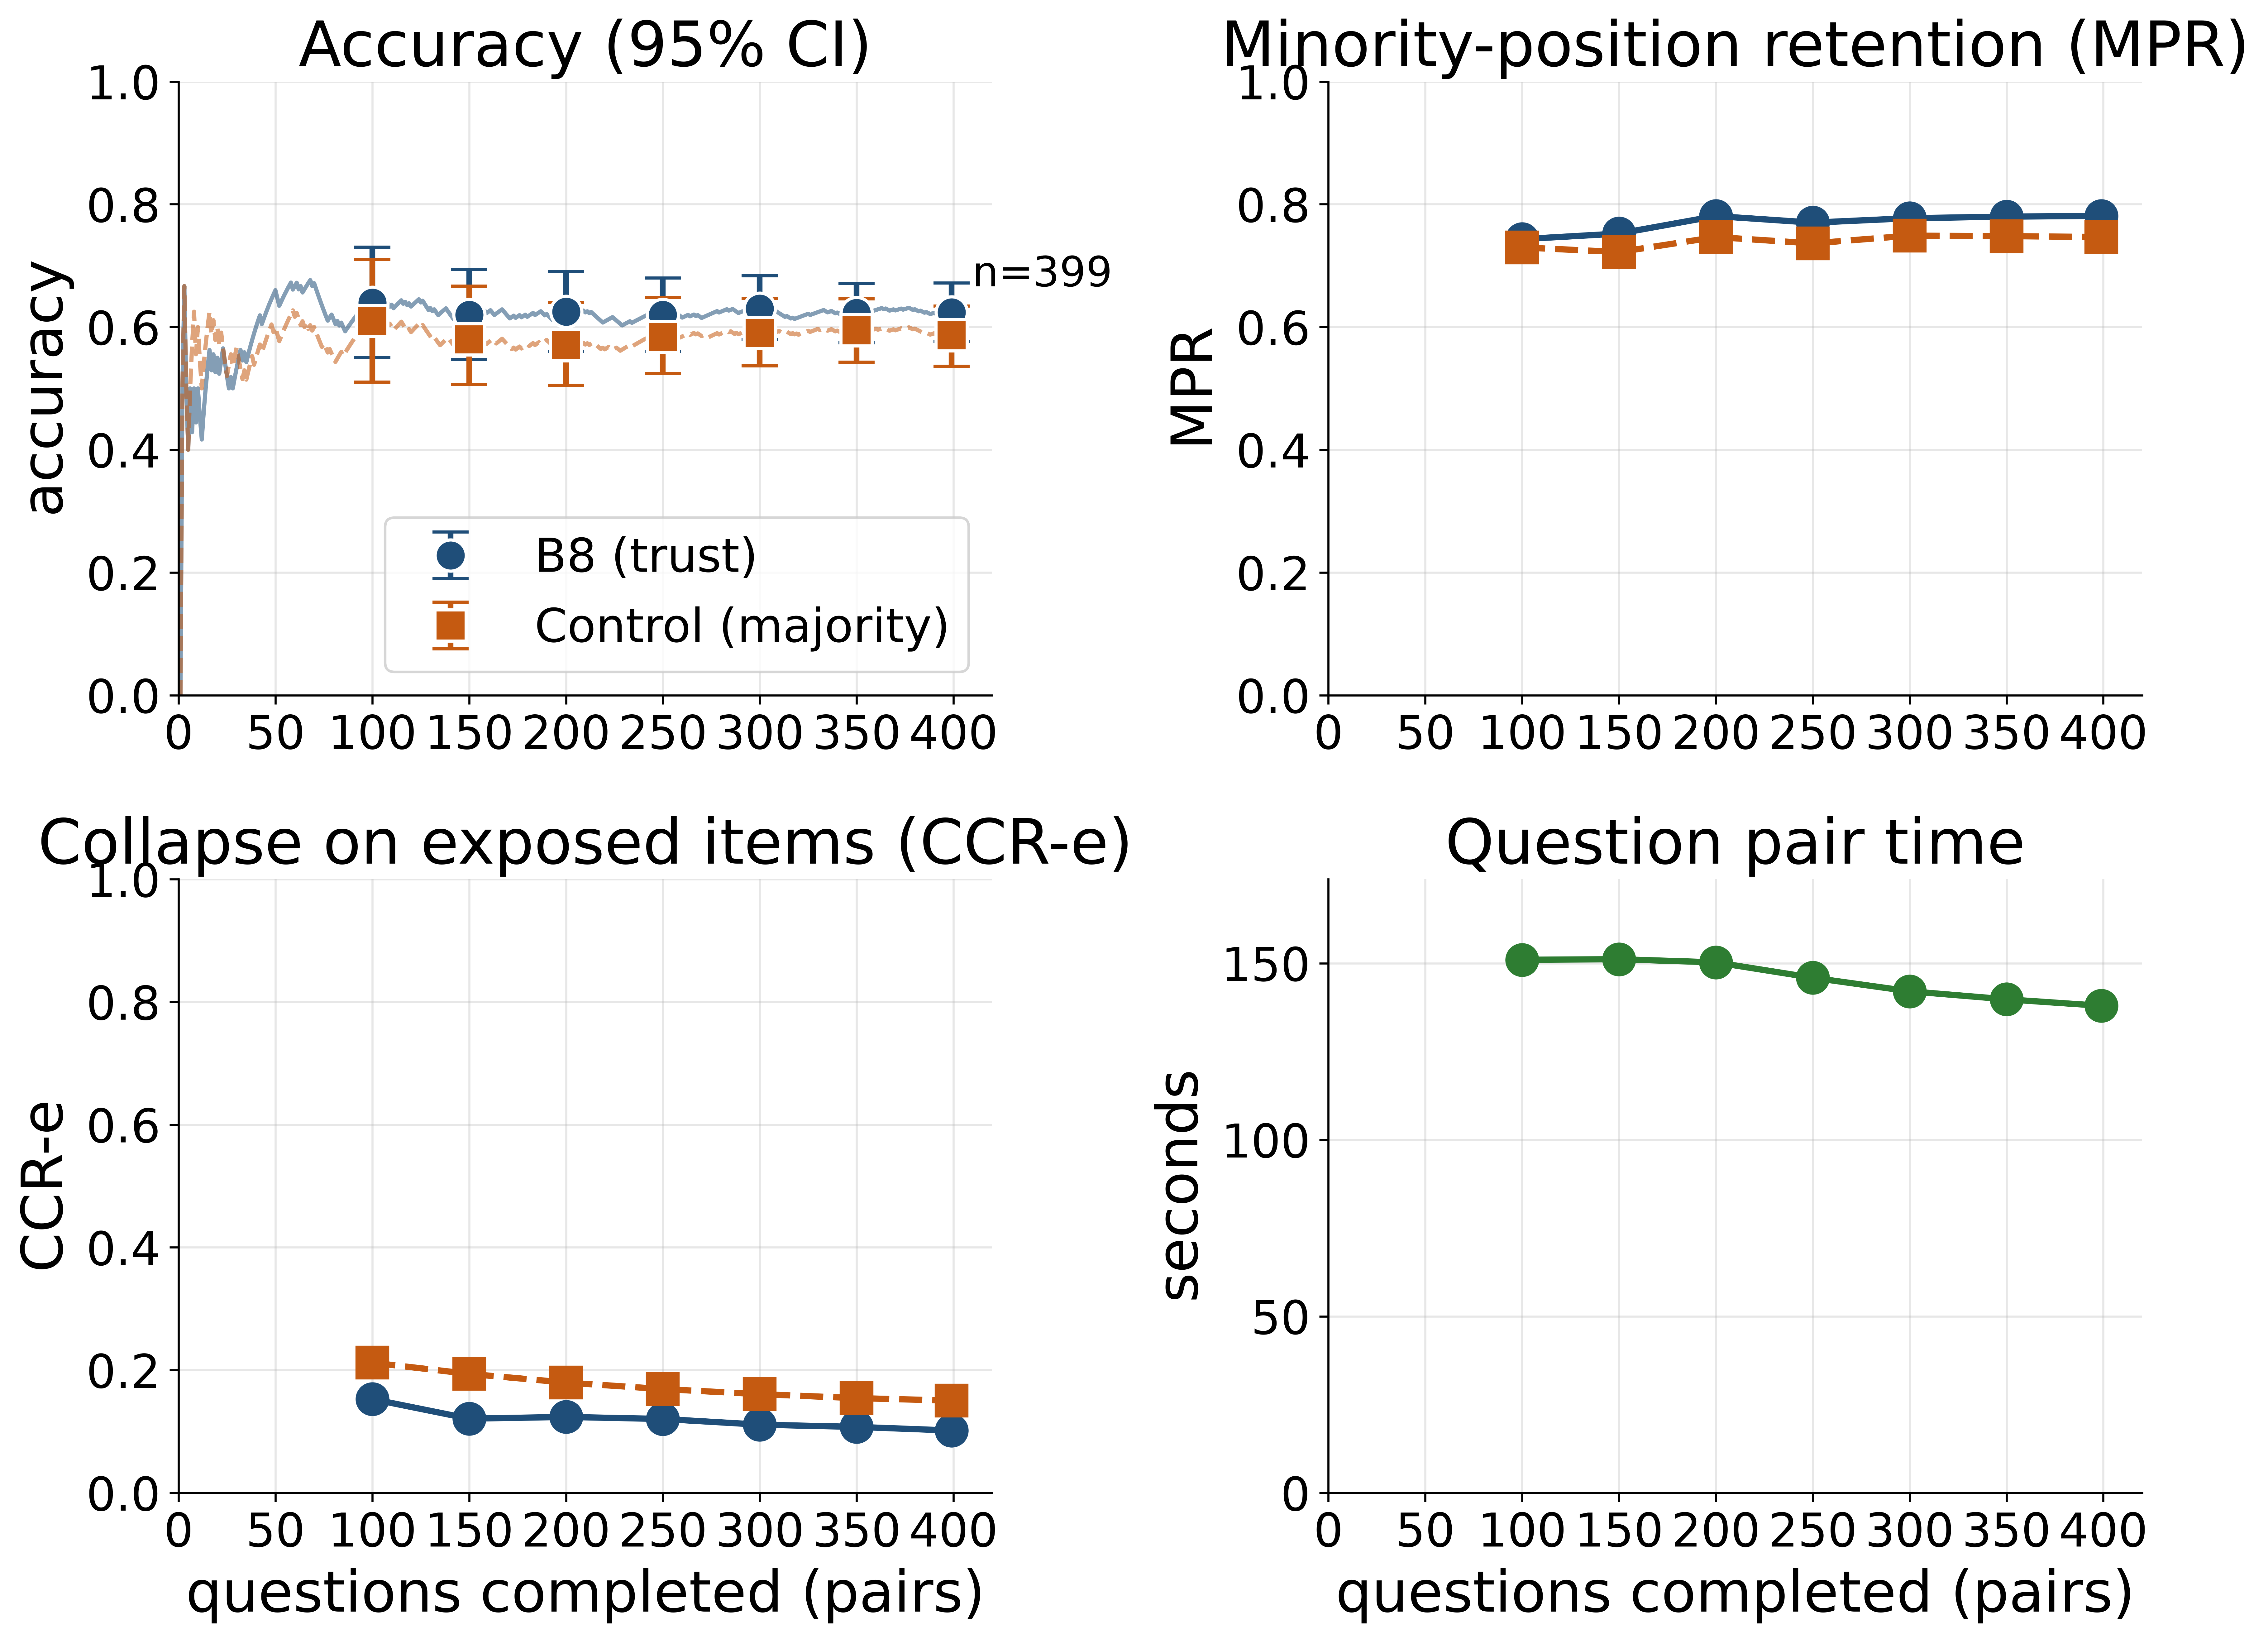
\includegraphics[width=\textwidth]{fig-core-results.png}
  \caption{First completed Core row (GPQA-Main, seed~1, 399 eligible pairs; question~27 quarantined). Top left: cumulative accuracy after each question (thin lines) with milestone snapshots and 95\% CIs (markers; B8 circles, control squares). Top right: minority-position retention (MPR) at milestones. Bottom left: collapse rate on evidence-exposed items (CCR-e). Bottom right: mean question-pair time in seconds. The B8 lead (+0.038 at $n=399$) is not significant (exact McNemar $p=0.086$); the figure is read as feasibility and timing evidence.}
  \label{fig:core-results}
\end{figure}

\paragraph*{Smoke results.}
Table~\ref{tab:core-smokes} collects the two hardware smokes that de-risked the row. The 4-bit N1a smoke served the full 53\,GB three-model stack on one 96\,GB card with every harness path running end to end. The FP8 smoke served the 73.68\,GB stack the same way after one config fix (4{,}096-token context, at most 16 concurrent sequences per server). Neither smoke is a finding: at $n=5$ the 4/5 versus 2/5 FP8 accuracy gap is noise in both directions.

\begin{table}[H]
  \centering
  \caption{4-bit N1a smoke (53\,GB stack, one 96\,GB card, 5 questions per arm). One injection item showed a transient effect the first check missed: the targeted agent moved under the injected consensus in round~2 and reverted by round~3; the check now detects any post-injection change. The oracle arm's fifth record was lost to a spot eviction, not to the pipeline.}
  \renewcommand{\arraystretch}{1.25}
  \small
  \begin{tabular}{|p{0.20\textwidth}|p{0.16\textwidth}|p{0.18\textwidth}|p{0.14\textwidth}|p{0.18\textwidth}|}
    \hline
    Arm & Records & Accuracy & MPR & Mean s/debate \\
    \hline
    B8 & 5/5 valid, 3 rounds & 0.40 (2/5) & 0.50 & 299.6 \\
    \hline
    Injection & 5/5 valid, 3 rounds & 0.80 (4/5) & 0.75 & 137.3 \\
    \hline
    B8-placebo & 5/5 valid, 3 rounds & 0.60 (3/5) & 0.75 & 258.1 \\
    \hline
    B8-oracle & 4/4 valid, 3 rounds & 1.00 (4/4) & --- & $\sim$280 \\
    \hline
  \end{tabular}
  \label{tab:core-smokes}
\end{table}

\begin{table}[H]
  \centering
  \caption{FP8 precision smoke (73.68\,GB stack, one 96\,GB card, same 5 questions as the 4-bit smoke). Mean 282.4\,s versus 299.6\,s: the same pace, so FP8 is a fidelity check, not a speed-up. FP8 endpoints: MPR 0.75, ARR 0.60, CCR-e 0.0.}
  \renewcommand{\arraystretch}{1.25}
  \small
  \begin{tabular}{|p{0.16\textwidth}|p{0.11\textwidth}|p{0.11\textwidth}|p{0.11\textwidth}|p{0.11\textwidth}|p{0.11\textwidth}|}
    \hline
    Stack & Q0 & Q1 & Q2 & Q3 & Q4 \\
    \hline
    4-bit (s) & 414.9 & 297.2 & 272.4 & 285.4 & 228.0 \\
    \hline
    FP8 (s) & 420.1 & 239.7 & 185.5 & 277.9 & 288.6 \\
    \hline
  \end{tabular}
  \label{tab:core-fp8}
\end{table}

\paragraph*{Discussion.}
The completed row supports a narrow conclusion: the full treatment and its matched control can be served together, run to completion, and scored on every pre-registered endpoint at about 138\,s per pair. It does not support a claim that trust-calibrated deliberation reduces sycophantic collapse. The paired gap is +3.8 points with $p=0.086$; the milestone snapshots never leave the 0.62--0.64 band for B8 against 0.57--0.61 for control, and every milestone $p$-value exceeds 0.05. A result in the design's expected direction at this $n$ is also consistent with noise, and the gap is below the pre-registered 7.5-point minimum detectable difference after Holm, so the study as designed cannot promote this row to an efficacy finding.

The trust signal itself is uninformative in this row. AUROC 0.518 on 69 agents is chance-level discrimination, and Brier 0.292 shows no calibration to exploit. The default verifier is lexical: support requires a shared term, so paraphrased evidence is missed and spurious overlap is rewarded, and the trust weights inherit both failures. The pre-registration treats verifier accuracy as a moderator for exactly this reason, and the 150--200-pair human audit is still outstanding; a matrix re-run under an audited verifier (cross-encoder or LLM judge) is the condition for any high-$q$ claim, not a cleanup step.

The secondary endpoints point the same way. B8 retains the correct minority slightly more often (MPR 0.78 versus 0.75) and collapses less often on evidence-exposed items (CCR-e 0.102 versus 0.150), but adapts less often when the majority is correct (ARR 0.657 versus 0.702): the trust weights add inertia in both directions. None of these contrasts is tested for significance in this report, the CCR-e denominators (128 and 153) are small, and the pressure arms are absent from this row, so the CMR and CCR denominators are empty and the collapse reading is exploratory. The optional B7 ceiling remains a reference, not a competitor: it answers what a strong single call gets on the same items, and it cannot replace the B8 versus B8-no-trust contrast.

\paragraph*{Threats to validity.}
The first threat is verifier quality. The lexical default can mistake a shared term for support, miss a negation, or misread a numeric claim. The cross-encoder is optional, and the NLI and LLM-judge paths are interfaces rather than validated components. LLM judges also show position, verbosity, and self-enhancement bias, so judge-based verifier outputs are treated as a measurement instrument rather than ground truth~\cite{zheng2023judging,wang2024large}. The human audit of 150--200 pairs is the gate that must pass before a high-$q$ claim. The second threat is retrieval coverage. The routing and deduplication logic are tested, but the live APIs are not; rate limits, malformed responses, and sparse domains can turn claims into unverifiable ones. The third threat is shared error. Three heterogeneous models reduce but do not eliminate correlated mistakes, and the shared-error floor bounds what any independent verifier can certify.

The fourth threat is benchmark gold. SciClaimBench is team-built, so its gold evidence and verdicts require annotation discipline and a defect-rate report. MMLU-Redux found errors in a substantial share of re-annotated MMLU questions, and human label variation is itself a known problem, so the SciClaimBench protocol treats adjudication and defect reporting as part of the measurement~\cite{gema2025mmulredux,plank2022labelvariation}. The fifth threat is model-family specificity: the result is conditional on the three chosen 4-bit checkpoints and the stack that served them. The sixth is stochasticity: the local models run at temperature 0.7, and the optional B7 ceiling uses three samples per question. The analysis averages over seeds where the design allows it and reports the variation that remains. The seventh is scope and compute. This row covers one dataset and one seed, so dataset and seed generality are untested; the pressure arms are absent, so CMR is unmeasurable and CCR-e is exploratory. The 4-bit trio has now served together on the 96\,GB card at a measured 138\,s per pair (about 15.3 GPU-hours for the row), but the 80\,GB A100 serving run is still pending, so a hardware change could still delay the remaining rows without changing the scientific question.

\section{Summary}\label{sec:implementation-summary}

The implementation is complete enough to run the debate loop, render and score multiple-choice options, decompose claims, route claims to domain-specific sources, update a bounded trust vector, aggregate a weighted answer, log a record, and validate the result schema. Gate~0 validates the base loop on ten GPQA questions. The P0 gate validates the wiring that Gate~0 did not cover, and the 615-test suite covers the contracts on synthetic and mock inputs. The first Core row adds the first comparative measurement: B8 at 0.6241 against 0.5865 for the matched majority control on 399 eligible GPQA-Main pairs, with exact McNemar $p=0.086$, MPR 0.78 versus 0.75, and an uninformative trust AUROC of 0.518. Those numbers are feasibility and timing evidence, not efficacy. The remaining work is the verifier human audit, the SciClaimBench calibration set, the WP-18 placebo/oracle slice, the second seed, and the remaining Core and Full rows. Those are the conditions for an efficacy claim, and none of them is met in this report.
